% Step 1: Set the \documentclass
\documentclass[draft]{agujournal2019}
\usepackage{url} %this package should fix any errors with URLs in refs.
\usepackage{lineno}
\usepackage[inline]{trackchanges} %for better track changes. finalnew option will compile document with changes incorporated.
\usepackage{soul}
\usepackage{graphicx}

\usepackage{upgreek}
\usepackage{textgreek}
\usepackage[greek,english]{babel}
\usepackage{subcaption}
\usepackage{adjustbox}
\usepackage{multirow}

\usepackage[final]{listings}
\usepackage{xcolor}
\definecolor{codeblue}{RGB}{19, 0, 255}
\definecolor{codegreen}{RGB}{0, 129, 0}
\definecolor{codegray}{rgb}{0.5,0.5,0.5}
\definecolor{codered}{RGB}{163, 21, 21}
\definecolor{backcolour}{rgb}{0.95,0.95,0.92}

\lstdefinestyle{mystyle}{
    backgroundcolor=\color{backcolour},
    commentstyle=\color{codegreen}, 
    keywordstyle=\color{codeblue}, 
    numberstyle=\tiny\color{codegray}, 
    stringstyle=\color{codered},
    basicstyle=\footnotesize, 
    columns=flexible,
    breakatwhitespace=false,
    breaklines=true,
    captionpos=b,
    keepspaces=true,
    numbers=left,
    numbersep=8pt,
    showspaces=false,
    showstringspaces=false,
    showtabs=false,
    tabsize=3}
\lstset{style=mystyle}

% Add these packages to stop hbox errors 
\vfuzz=100pt 
\hfuzz=100pt 
\usepackage{etoolbox}
\apptocmd{\sloppy}{\hbadness 10000\relax}{}{}

\linenumbers

%%%%%%%
% As of 2018 we recommend use of the TrackChanges package to mark revisions.
% The trackchanges package adds five new LaTeX commands:
%  \note[editor]{The note}
%  \annote[editor]{Text to annotate}{The note}
%  \add[editor]{Text to add}
%  \remove[editor]{Text to remove}
%  \change[editor]{Text to remove}{Text to add}
% complete documentation is here: http://trackchanges.sourceforge.net/
%%%%%%%

\draftfalse

%% Enter journal name below.
%% Choose from this list of Journals:
% JGR: Atmospheres; JGR: Biogeosciences; JGR: Earth Surface; JGR: Oceans; JGR: Planets; JGR: Solid Earth Geophysical Research Letters; Reviews of Geophysics; Tectonics; Geochemistry, Geophysics, Geosystems

\journalname{Default: Geochemistry, Geophysics, Geosystems}

\begin{document}

\graphicspath{{Figures/}}

%% ------------------------------------------------------------------------ %%
%  Title
% (A title should be specific, informative, and brief. Use abbreviations only if they are defined in the abstract. Titles that start with general keywords then specific terms are optimized in searches)
\title{PyBaselines: An Open-Source MCMC Algorithm for Fitting Baselines to FTIR Spectra of Basaltic-Rhyolitic Glasses}
%% ------------------------------------------------------------------------ %%

%% ------------------------------------------------------------------------ %%
%  AUTHORS AND AFFILIATIONS
%% ------------------------------------------------------------------------ %%

% Authors are individuals who have significantly contributed to the research and preparation of the article. Group authors are allowed, if each author in the group is separately identified in an appendix.)

\authors{Sarah Shi\affil{1, 4}, Henry Towbin\affil{1}, Terry Plank\affil{1}, Anna Barth\affil{1, 2}, Dan Rasmussen\affil{1, 3}}
\affiliation{1}{Lamont-Doherty Earth Observatory, Columbia University. New York, NY USA}
\affiliation{2}{University of California, Berkeley. Berkeley, CA USA}
\affiliation{3}{National Museum of Natural History, Smithsonian Institution. Washington, DC USA}
\affiliation{4}{University of Cambridge}

%% Corresponding Author: Corresponding author mailing address and e-mail address. 
\correspondingauthor{Sarah Shi}{scs2202@columbia.edu}

%% Keypoints, final entry on title page. List up to three key points (at least one is required). Key Points summarize the main points and conclusions of the article. Each must be 140 characters or fewer with no special characters or punctuation and must be complete sentences

\begin{keypoints}
\item 1
\item 2
\end{keypoints}

%% ------------------------------------------------------------------------ %%
%  ABSTRACT and PLAIN LANGUAGE SUMMARY. 
% A good Abstract will begin with a short description of the problem being addressed, briefly describe the new data or analyses, then briefly states the main conclusion(s) and how they are supported and uncertainties.

% The Plain Language Summary should be written for a broad audience, including journalists and the science-interested public, that will not have a background in your field. A Plain Language Summary is required in GRL, JGR: Planets, JGR: Biogeosciences, JGR: Oceans, G-Cubed, Reviews of Geophysics, and JAMES. see http://sharingscience.agu.org/creating-plain-language-summary/)

%% ------------------------------------------------------------------------ %%
%  ABSTRACT

\begin{abstract}

\end{abstract}
%% ------------------------------------------------------------------------ %%



%% ------------------------------------------------------------------------ %%
%  PLAIN LANGUAGE SUMMARY

% \section*{Plain Language Summary}

%% ------------------------------------------------------------------------ %%



%% ------------------------------------------------------------------------ %%
%  INTRODUCTION 

\section{Introduction} 

Degassing of volatiles in magmas modulate magma phase equilibria~\cite{SissonandGrove1993}, crystallinity~\cite{BlundyandCashman2001}, density~\cite{OchsandLange1999}, and viscosity~\cite{HessandDingwell1996} from generation to eruption. The most abundant of these volatiles are H$_2$O and CO$_2$, both of which dissolve in silicate melts with strong pressure dependence. Analyses of H$_2$O and CO$_2$ in melt inclusions trapped in mineral crystals can thus be utilized to estimate the conditions of magma storage and evolution, whereas those in experimental charges inform understandings of solubility and phase equilibria. H$_2$O and CO$_2$ in volcanic glasses are commonly measured with the two analytical techniques of Fourier Transform Infrared Spectroscopy (FTIR) and Secondary-Ion Mass Spectrometry (SIMS) to characterize natural volcanic systems and experimental recreations of high-pressure and high-temperature magmatic conditions. \textbf{\textit{necessary to talk a bit about benefits and drawbacks here? or later?}}

FTIR spectroscopy excites materials with visible light through wavelengths in the infrared region to determine transitions in rotational, vibrational, and electronic energies. Volatiles in silicate glasses absorb light proportional to concentration in certain wavelength regions, allowing for recognition and quantification of species with the Beer-Lambert Law: 
\begin{equation}
c = \frac{A M}{\varepsilon l \rho}
\end{equation}
where $c$ is concentration, $A$ is absorbance, $M$ is the molar mass of the absorbing volatile species (g$\cdot$mol$^{-1}$), \textepsilon{} is the absorptivity of the species (L$\cdot$mol$^{-1}\cdot$ cm), $l$ is the optical path length or thickness (cm), and \textrho{} is density (kg$\cdot$m$^{-3}$). \textbf{Provide image of spectrum, define IR near IR regions, describe a bit.} 

Linear relationships between absorbance and concentration dominate, but non-linear relationships can be introduced when increased sample thicknesses result in insufficient light transmission to the detector, pushing peaks to become saturated as with the ${\mathrm{H_2O_{t, 3550}}}$ peak~\cite{McIntoshetal2017, vonAulocketal2014}. The ${\mathrm{H_2O_{t, 3550}}}$ peak can be well quantified with a linear to near-linear baseline between the two absorbance minima on either side of peak when the peak is unsaturated with a raw absorbance of \textless 2 ~\cite{DixonandStolper1995, vonAulocketal2014}. When \textepsilon${\mathrm{H_2O_{t, 3550}}}$ is saturated, the combination of H$_{2}$O$_{\mathrm{m}, 5200}$ or the H$_{2}$O$_{\mathrm{m}, 1635}$ and the OH$^{-}_{4500}$ must be used instead. 

Volatile concentrations in silicate glasses require the measurement of peak heights or areas, by measuring the difference in absorbance or integrated absorbance between peak and baseline. Variability and subjectivity in baseline definition constitutes a significant uncertainty in studies determining volatile concentrations, from inception to present. The H$_{2}$O$_{\mathrm{m}, 5200}$, OH$^{-}_{4500}$, and \textepsilon${\mathrm{H_2O_{t, 3550}}}$ peaks in the near-infrared (12800-4000 cm$^{-1}$) to mid-infrared (4000-200 cm$^{-1}$) region can be well quantified with linear to near-linear baselines between the two absorbance minima on either side of the peak. The H$_{2}$O$_{\mathrm{m}, 1635}$ peak and CO$_{3}^{2-}$ doublet peaks pose greater challenges due to the steep and sharp increase of baseline absorbance at wavenumbers lower than 1430 cm$^{-1}$. Furthermore, the convolution of the tails of the H$_{2}$O$_{\mathrm{m}, 1635}$ and the CO$_{3}^{2-}$1515 doublet peak in melt inclusion spectra further complicates the appropriate baselines in the near infrared region. Baselines beneath the H$_{2}$O$_{\mathrm{m}, 1635}$ and CO$_{3}^{2-}$ doublet peaks have been approximated with the spectra of matrix- and chemistry-matched devolatilized glasses~\cite{Dixonetal1988, Newmanetal2000}, splines and flexicurves~\cite{DixonandStolper1995}, and other curve functions~\cite{DixonandClague2001}. Devolatilized glass baselines are the gold standard but are not possible in melt inclusion studies, where large pieces of glass are not readily available. Spline, flexicurve, and curve function baselines generated without open-source code are not replicable and not associated with appropriate uncertainties. 

We examine each parameter within the Beer-Lambert Law to develop PyBaselines, a Python implementation of a Bayesian-informed Multi-Core Markov Chain Monte Carlo algorithm for fitting baselines and peaks for all H$_2$O and CO$_2$ species. We assess the fundamental shape and variability of the baseline using principal component analysis (PCA) applied to a database of absorbance spectra for volatile-free and volatile-poor melt inclusions from the Aleutian arc~\cite{RasmussenThesis} and MORB glasses~\cite{Newmanetal2000}. This dataset of naturally devolatilized spectra is relevant for basaltic to rhyolitic silicate melts. The application of PCA to a training dataset of devolatilized spectra allows for the assessment of the fundamental shape of the baseline and the spectral features contributing to variability~\cite{Carvajaletal2016}. We refit the relationships between molar absorptivity and composition with implicit iterative inversion with updated datasets from the last parameterization of~\citeA{Mandevilleetal2002} and to derive molar absorptivity with uncertainty. We develop automated implementations for calculating thicknesses from reflectance spectra by the reflectance FTIR interference fringe method. PyBaselines allows for the reproducible quantification of volatile concentrations with meaningful uncertainties.

%% ------------------------------------------------------------------------ %%



%% ------------------------------------------------------------------------ %%
\section{Background}
\subsection{Fourier Transform Infrared Spectroscopy (FTIR) Background}
I currently have everything incorporated into computational methodology -- both background and our solutions. This is a lot of the structural trouble I was thinking about. I don't really know to split this well. How to split??????????????????????????

Nonlinearities, linear 
Species dependent dissolution, etc. 
Peak appearances 

%  When \textepsilon${\mathrm{H_2O_{t, 3550}}}$ is saturated, the combination of H$_{2}$O$_{\mathrm{m}, 5200}$ or the H$_{2}$O$_{\mathrm{m}, 1635}$ and the OH$^{-}_{4500}$ must be used instead. The H$_{2}$O$_{\mathrm{m}, 5200}$ and OH$^{-}_{4500}$ peaks can be fit with a linear to near-linear baseline, or a baseline consisting of two Gaussians~\cite{Ohlhorstetal2001, Stabileetal2020, Stolper1982, WithersandBehrens1999}. The linear to near-linear baseline is advantageous given the reproducibility of peak heights but can underestimate the peak height or area given the presence of iron and water-related bands ($\sim$5700 and $\sim$4000 cm$^{-1}$, respectively) in dacitic to basaltic compositions~\cite{Ohlhorstetal2001}. The species concentration of H$_{2}$O$_{\mathrm{m}, 5200}$ and OH$^{-}_{4500}$ by the two Gaussian method agrees well with NMR spectroscopy but is highly sensitive to raw absorbance and can be difficult to reproduce across studies~\cite{Ohlhorstetal2001}. The \textepsilon${\mathrm{H_2O_{t, 3550}}}$, H$_{2}$O$_{\mathrm{m}, 5200}$, and OH$^{-}_{4500}$ baselines are thus fit with the asymmetric least squares (ALS) method, iteratively solving for an interpolated fitting which balances smoothness and asymmetry~\cite{Eilers2004, Leeetal2017, Pengetal2010}

%% ------------------------------------------------------------------------ %%
%  COMPUTATIONAL METHODOLOGY 

\section{Computational Methodology} % Section - 1.4

%  ASSESSING VARIABILITY IN THE BASELINE
\subsection{Assessing Variability in Baselines and Peaks}
The shape and variability of the baseline and the $\mathrm{H_2O_{m, 1635}}$ and CO$_{3}^{2-}$ peaks were assessed with a database of $\sim$90 absorbance FTIR spectra for Aleutian melt inclusions and MORB glasses \textbf{\textit{need Henry's numbers for each type of spectrum, statistics on composition, data to upload to Github repository -- Henry is collaborator so can maybe post a new directory about all this with code}}. The spectra variably lack CO$_{3}^{2-}$ (decarbonated), $\mathrm{H_2O_{m, 1635}}$ (dehydrated), or both CO$_{3}^{2-}$ and $\mathrm{H_2O_{m, 1635}}$ (devolatilized) and span a wide compositional range (SiO$_2$ = 43-60 wt.\%, MgO = 2.1-6.4 wt.\%, Na$_2$O = 2.2-4.3 wt.\%, K$_2$O = xy value). 

Definition of baseline and peak shapes was iterative. Completely devolatilized absorbance spectra were scaled and shifted to ensure equal absorbances in the fitting range from 2400 to 1275 cm$^{-1}$. We first generate the initial mean baseline ($\mathrm{\overline{Baseline}_i}$) and described variability within the baseline with principal component analysis (PCA). Four principal components describe $\ge$ 95\% of the variance within the baseline. 

\begin{figure}[htb!] 
\centering
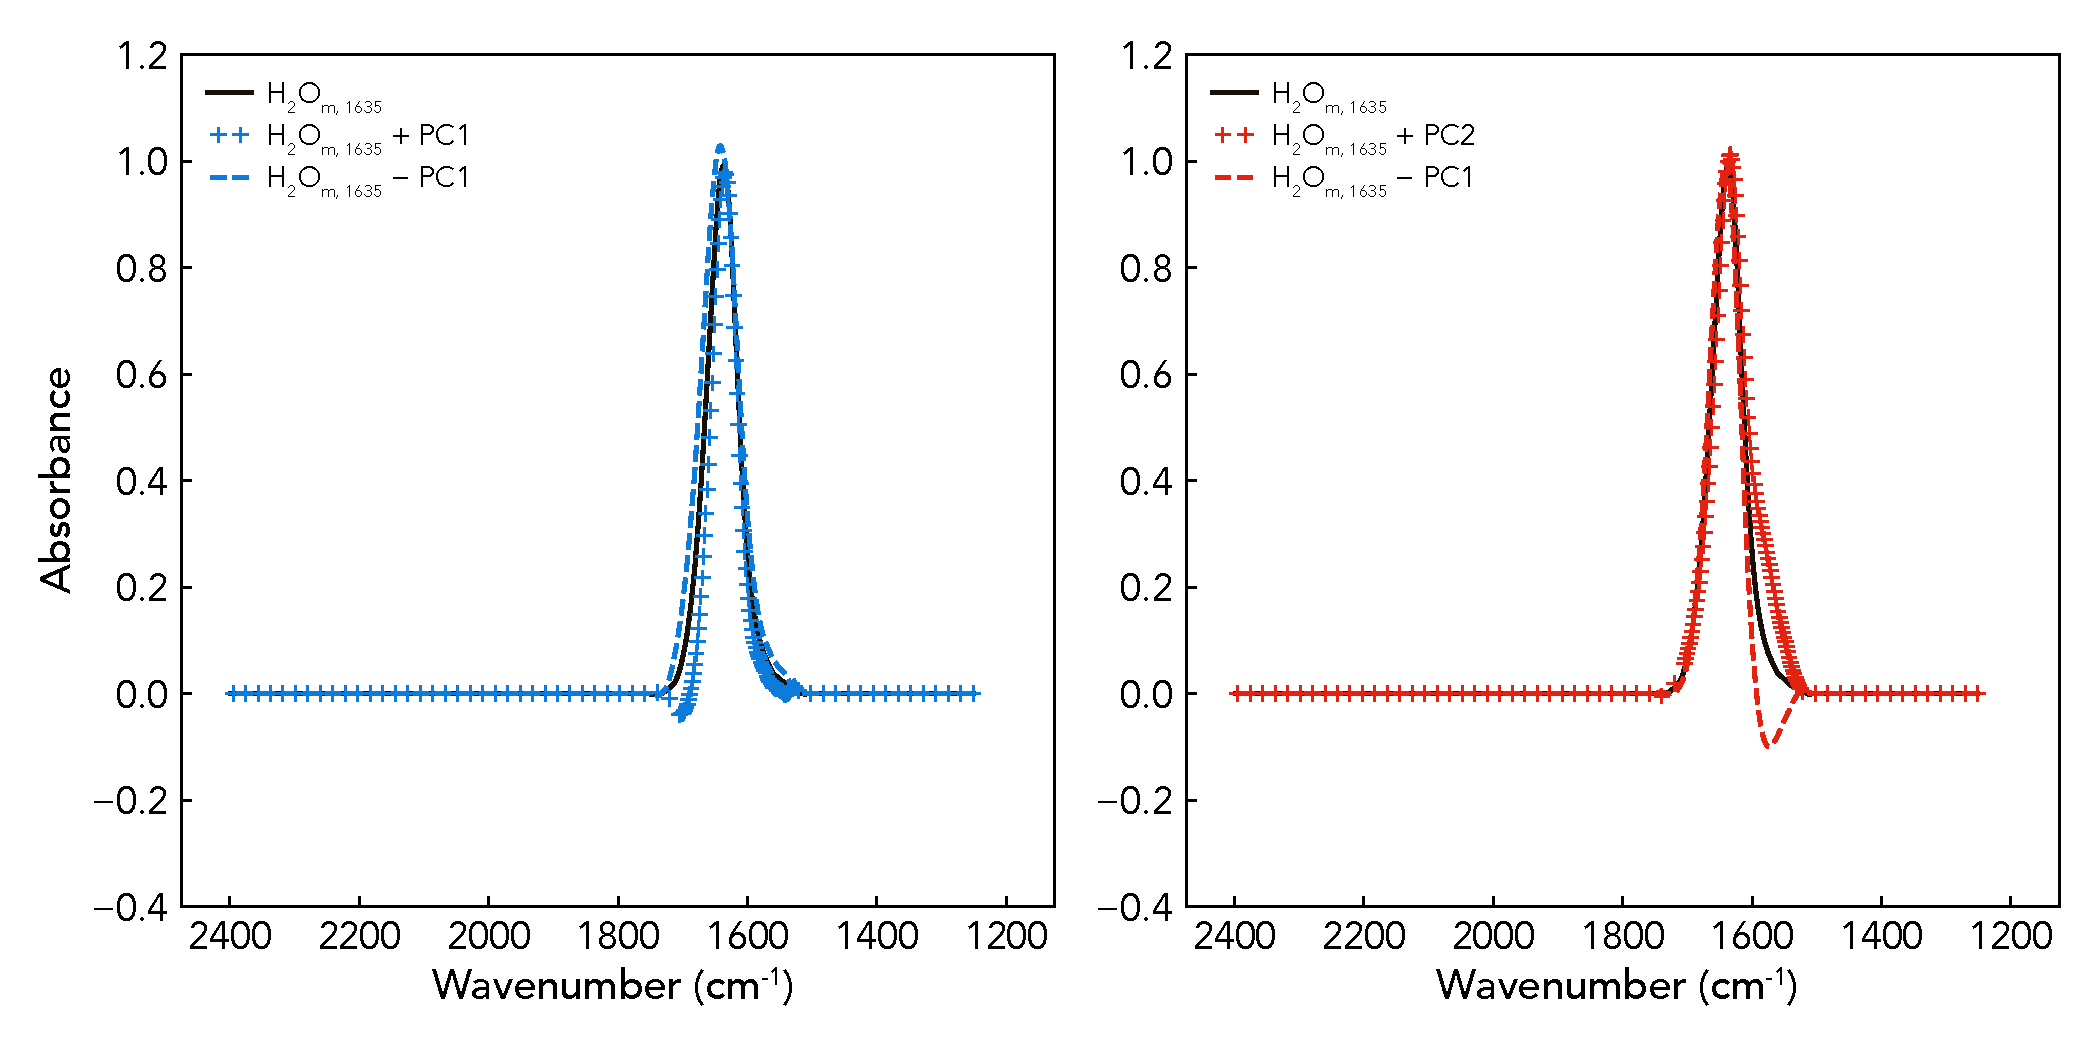
\includegraphics[width=1.0\textwidth]{H2Om1635+PCVectors_Subplot}
\caption[Mean $\mathrm{H_2O_{m, 1635}}$ peak with PC components describing variability]{Mean $\mathrm{H_2O_{m, 1635}}$ peak with PC components describing variability}
\label{figure:H2OmwithPCA}
\end{figure}    

Decarbonated spectra containing only $\mathrm{H_2O_{m, 1635}}$ peaks were fit with the $\mathrm{\overline{Baseline}_i}$ and two principal components to isolate the shape of the $\mathrm{H_2O_{m, 1635}}$ peak, which is neither Gaussian nor Lorentzian peaks. We thus identify the mean $\mathrm{H_2O_{m, 1635}}$ ($\mathrm{\overline{H_2O_{m, 1635}}}$) peak shape and describe variability within the peak with PCA (Figure~\ref{figure:H2OmwithPCA}). The downturn of the $\mathrm{H_2O_{m, 1635}}$ peak occurs more rapidly than that of a Gaussian or Lorentzian peak \textbf{\textit{Maybe need a figure from Henry to show our proof of this}}. Principal components (PC) 1 and 2 allow for slight lateral deviations of the $\mathrm{H_2O_{m, 1635}}$central  peak location, generating better fits when shifted away from the standard peak location at 1635 cm$^{-1}$. Two principal components describe $\ge$ 95\% of the variance within the baseline. Identification of the $\mathrm{H_2O_{m, 1635}}$ peak shape further allows for $\mathrm{H_2O_{m, 1635}}$ peak subtraction from the decarbonated spectra with least squares, generating additional devolatilized spectra. 

Dehydrated spectra with CO$_{3}^{2-}$ were similarly utilized to describe the CO$_{3}^{2-}$ peaks, which are simple Gaussian peaks \textbf{\textit{Maybe need a figure from Henry to show our proof of this}}. CO$_{3}^{2-}$ peak subtraction from dehydrated spectra with least squares generate more devolatilized spectra.

Decarbonated and dehydrated spectra were thus converted to entirely devolatilized spectra. We iteratively identify and iteratively define the mean devolatilized baseline ($\mathrm{\overline{Baseline}}$) with associated variability (Figure~\ref{figure:BaselinewithPCA}). Variability in the baseline can be described with the addition or subtraction of these PC components, highlighting and describing the different baselines observed within the devolatilized spectrum database. We further disentangle the convoluted tails of the overlapping $\mathrm{H_2O_{m, 1635}}$ and the CO$_{3, 1515}^{2-}$ peaks by identifying $\mathrm{\overline{H_2O_{m, 1635}}}$ with associated principal components and the Gaussian nature of the CO$_{3}^{2-}$ peaks. Given the sharp upturn in absorbance while approaching 1275 cm$^{-1}$, we provide additional accomodation for shifting and tilting the $\mathrm{H_2O_{m, 1635}}$ and CO$_{3, 1515}^{2-}$ peaks with a linear shift. We can therefore credibly describe the range of possible devolatilized baselines while simultaneously fitting peaks appropriate for basaltic-rhyolitic glasses with the net equation: 
\begin{equation}
    \hat{A} = \hat{B} + \hat{\mathrm{H_2O_{m, 1635}}} + \hat{\mathrm{CO_{3}^{2-}}} + \hat{L}, 
\end{equation}
where $\hat{A}$ is the best-fit absorbance spectrum. 
$\hat{B}$ or the best-fit baseline is: 
\begin{equation}
    \hat{B} = x_0 \overline{B} + x_1 \overline{B}_{PC1} + x_2 \overline{B}_{PC2} + x_3 \overline{B}_{PC3} + x_4 \overline{B}_{PC4}, 
\end{equation}
where the $x_{subscript}$ terms are best-fit scaling parameters, $\overline{B}$ is the mean baseline, and $\overline{B}_{PC}$ is the n-th principal component of the baseline. 
$\hat{\mathrm{H_2O_{m, 1635}}}$ or the best-fit $\mathrm{H_2O_{m, 1635}}$ peak is: 
\begin{equation}
    \hat{\mathrm{H_2O_{m, 1635}}} = y_0 \overline{H_2O_{m, 1635}} + y_1 \overline{H_2O_{m, 1635}}_{PC1} + y_2 \overline{H_2O_{m, 1635}}_{PC2}, 
\end{equation}
where the $y_{subscript}$ terms are best-fit scaling parameters, $\overline{H_2O_{m, 1635}}$ is the mean $H_2O_{m, 1635}$ peak, and $\overline{H_2O_{m, 1635}}_{PC}$ is the n-th principal component of the $H_2O_{m, 1635}$ peak. Peak amplitude is fit with $\overline{H_2O_{m, 1635}}$ and the principal components accomodate variations in peak location. 
$\hat{CO_{3, 1515/1430}^{2-}}$ or the best-fit CO$_{3}^{2-}$ peak is: 
\begin{equation}
    \hat{CO_{3, 1515/1430}^{2-}} = \frac{a}{2\sigma^2} \cdot e^{-(\upsilon^- - \mu)^2},
\end{equation}
where $a$ is the amplitude, $\sigma$ is the peak half-width, \textupsilon$^-$ is the wavenumber range of 2400 to 1275 cm$^{-1}$, and $\mu$ is the central wavenumber of the peak. The $\mu$ paraemter accounts for slight deviations in peak location. 
$\hat{L}$ or the best-fit line accomodating for shifting and tilting of peaks is: 
\begin{equation}
    \hat{L} = mv + b 
\end{equation}
where m is the slope, $v$ is the wavenumber range of interest, and b is the intercept. 

\begin{figure}[htb!] 
\centering
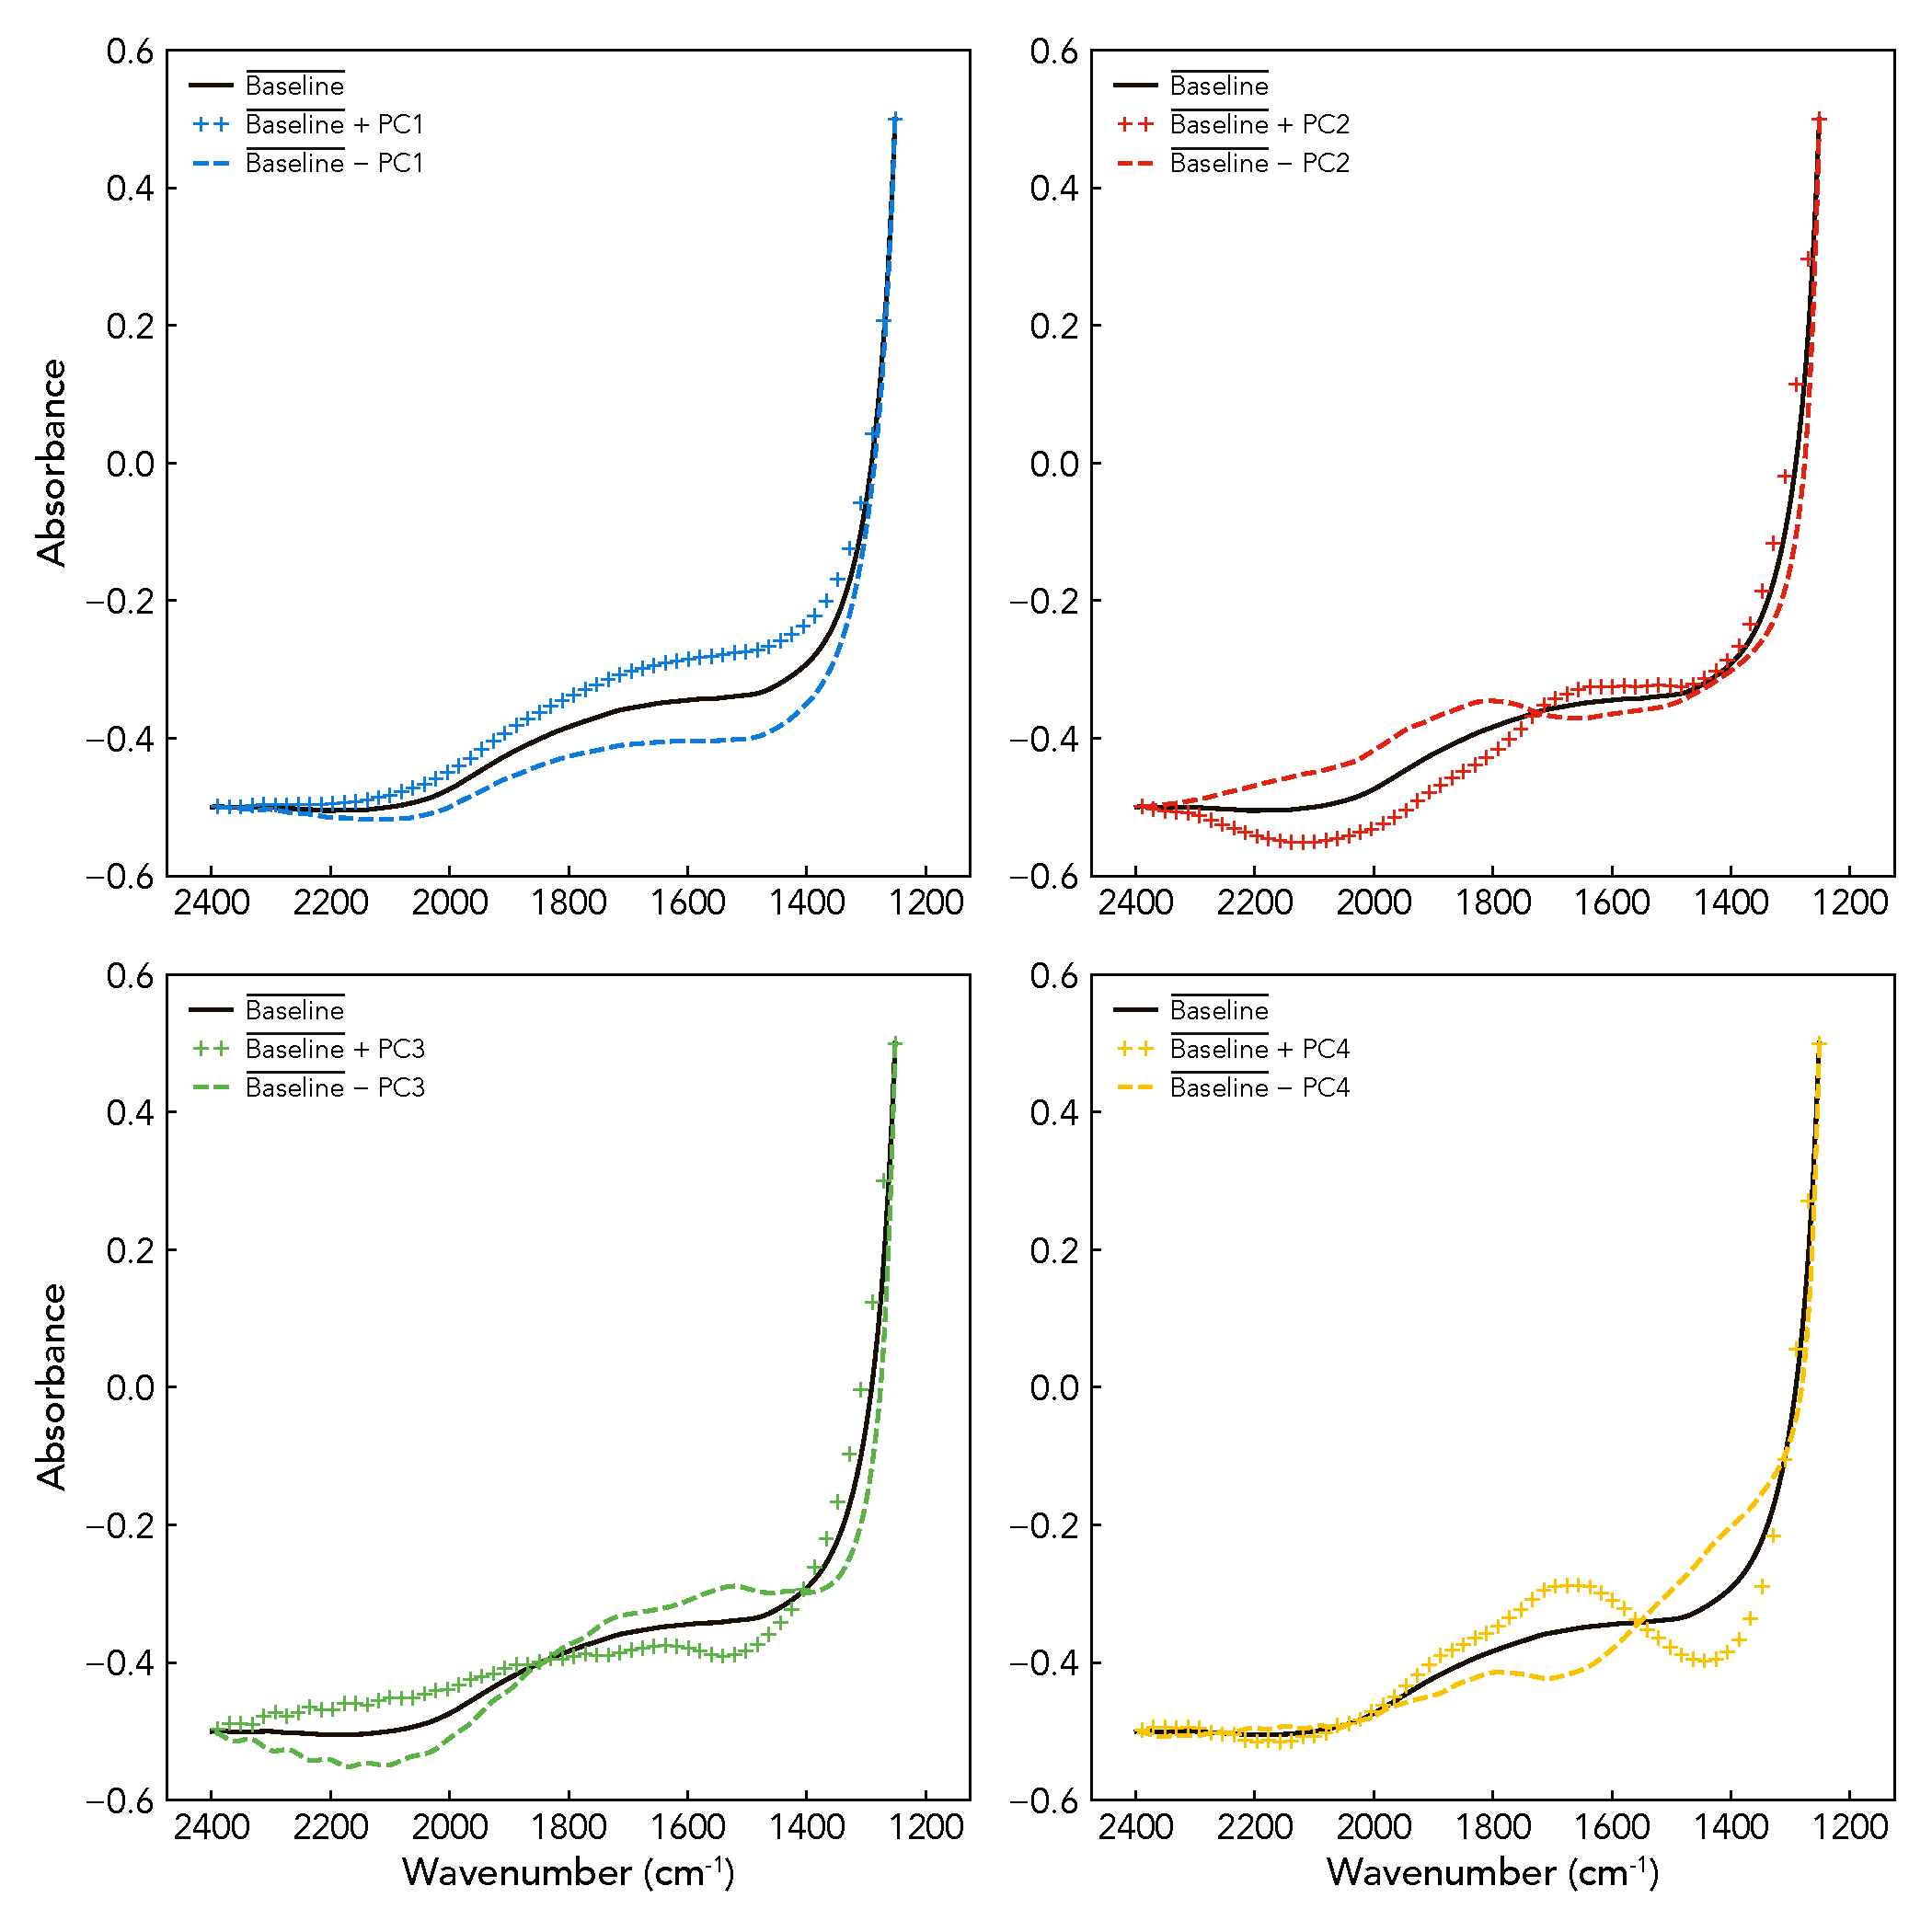
\includegraphics[width=1.0\textwidth]{BL+PCVectors_Subplot}
\caption[Mean devolatilized baseline with PC components describing variability]{Mean devolatilized baseline ($\overline{}$) with PC components describing potential variability within the basleine. A. }
\label{figure:BaselinewithPCA}
\end{figure}

%  CALIBRATING MOLAR ABSORPTIVITY
\subsection{Calibrating Molar Absorptivity (\textepsilon)}
Molar absorptivities or extinction coefficients (\textepsilon) determine the intensity at which light attenuates when passing through a material and relates absorbance to concentration, calibrated by pairing analyses of volatile content by transmission FTIR and by an additional independent analytical technique. \textepsilon is dependent on glass composition, related to both the tetrahedral cation fraction of $\uptau$=(Si$^{4+}$+Al$^{3+}$)/(total cations) and the cation fraction of Na$^{+}$/(Na$^{+}$+Ca$^{2+}$). The \textepsilon data are limited to studies with independent methods of volatile measurement – such as SIMS, Karl Fischer titration, experimental mass balance, vacuum heating, or manometry – and with H$_{2}$O $>$ 0.5 wt.\% for peak resolution. In the full dataset, $\uptau$ spans the range of 0.50-0.90 and Na$^{+}$/(Na$^{+}$+Ca$^{2+}$) from 0.23-0.84. We examine whether these compositional parameters remain the best descriptors of extinction coefficient. We refit the linear relationships between \textepsilon${\mathrm{CO_3^{2-}}}$, \textepsilon${\mathrm{OH^{-}_{4500}}}$, \textepsilon${\mathrm{H_2O_{t, 3550}}}$, \textepsilon${\mathrm{H_2O_{m, 1635}}}$, and \textepsilon${\mathrm{CO_3^{2-}}}$ and the corresponding compositional parameters values to include more recent data and broader compositional ranges since the last compilation of extinction coefficients by~\citeA{Mandevilleetal2002}, with an implicit inversion. 

The extinction coefficients related to H$_2$O species increase with tetrahedral cation fraction, $\uptau$, reflecting increased polymerization of the glass~\cite{Stolper1982}. Tetrahedral cations have also been proposed to compete with non-tetrahedral cations (M = Mg$^{2+}$, Ca$^{2+}$, Na$^{+}$) to bond with free hydroxyl groups in melt~\cite{Mercieretal2010, Pandyaetal1992}. More depolymerized melts will have higher proportions of free hydroxyl, which translates to more M-(OH)$_x$ bonding and hydrogen bonding~\cite{Mercieretal2010, Xue2009}.~\citeA{Dixonetal1995} and~\citeA{Mandevilleetal2002} demonstrate the dependence of the \textepsilon${\mathrm{H_2O_{m, 5200}}}$, \textepsilon${\mathrm{OH^{-}_{4500}}}$, and \textepsilon${\mathrm{H_2O_{m, 1635}}}$ on glass tetrahedral cation fraction. Tetrahedral cation fraction is similarly observed to be positively correlated with \textepsilon${\mathrm{H_2O_{t, 3550}}}$, but this relationship is less straightforward~\cite{Mercieretal2010}. Quench temperatures and quench rates drive the formation of variable proportions of H$_{2}$O$_{\mathrm{m}}$ and OH$^{-}$~\cite{SilverandStolper1989, Stolper1989}. \textepsilon${\mathrm{H_2O_{t, 3550}}}$ is thus considered as a combination of two endmember absorption coefficients, \textepsilon${\mathrm{OH^{-}_{3550}}}$ and \textepsilon${\mathrm{H_2O_{m, 3550}}}$, multiplied by the relative proportion of each respective species~\cite{McIntoshetal2017, Newmanetal1986, Okumuraetal2003}. Studies quantifying \textepsilon${\mathrm{OH^{-}_{3550}}}$ and \textepsilon${\mathrm{H_2O_{m, 3550}}}$ are the gold standard, but are currently limited in compositional range;~\citeA{McIntoshetal2017} considered the range of $\uptau$ = 0.746-0.800, spanning silicic compositions from rhyolitic to albitic glasses. More experiments are needed to properly quantify the species-dependent nature of the $\mathrm{H_2O_{t, 3550}}$ peak. We find a positive relationship between \textepsilon${\mathrm{H_2O_{t, 3550}}}$ and $\uptau$, despite compilations presented by speciation. While endmember data for H$_{2}$O$_{\mathrm{t, 3550}}$ remain limited, \textepsilon${\mathrm{H_2O_{t, 3550}}}$ is best described by $\uptau$. The relationship observed with NBO/T, calculated by methods outlined in~\citeA{MysenandRichet2018}, is not observed in this dataset, despite the observation in~\citeA{Mercieretal2010} (Supplemental Figure xx). 

~\citeA{DixonandPan1995} first demonstrate the dependence of the CO$_{3}^{2-}$ doublet absorption coefficients on the molar or cationic ratio of Na$^{+}$/(Na$^{+}$+Ca$^{2+}$). The proportion of Na$^{+}$ to Ca$^{2+}$ modulates the dissolution of C as molecular CO$_{2}$ and/or CO$_{3}^{2-}$. As the proportion of Ca$^{2+}$ increases, \textepsilon${\mathrm{CO_3^{2-}}}$ decreases. C dissolves as both molecular CO$_{2}$ and CO$_{3}^{2-}$ in NaAl-rich silicate glasses (albitic, jadeitic, nephelinitic compositions)~\cite{DixonandPan1995, FineandStolper1985, MysenandVirgo1980a, MysenandVirgo1980b}. C solely dissolves as CO$_{3}^{2-}$ in Ca and CaMg-rich silicate glasses (diopsidic, sodamelilitic, and akermanitic compositions)~\cite{DixonandPan1995, FineandStolper1986}. \textepsilon${\mathrm{CO_3^{2-}}}$ data are often limited to either the \textepsilon${\mathrm{CO_{3, 1515}^{2-}}}$ or \textepsilon${\mathrm{CO_{3, 1430}^{2-}}}$ peak, which are also assumed to be approximately equal~\cite{DixonandPan1995}. A cumulative \textepsilon${\mathrm{CO_3^{2-}}}$ is fit with data from \textepsilon${\mathrm{CO_{3, 1515}^{2-}}}$ or \textepsilon${\mathrm{CO_{3, 1430}^{2-}}}$, where available, given the variability in the baseline fitting method. 

Uncertainties exist within both the compositional parameter and the quantification of \textepsilon. Variability in compositional parameters may exist in older experimental studies where microprobe measurements quantify limited oxides. Variability in \textepsilon can be attributed to variability in the baseline fitting method. H$_{2}$O$_{\mathrm{m}, 5200}$ and \textepsilon${\mathrm{OH^{-}_{4500}}}$ have been quantified with both linear and Gaussian baselines, resulting in likely differences in the determined absorption coefficient. The inversion applies Newton’s method for determining the minimum of a function in a non-linear inverse problem. The Newtonian inversion derives strength from the ability to incorporate experimental and compositional uncertainties into the calibration and to utilize information on the shape of the error for a trial solution to successively derive improved fits for model parameters which minimize error. We apply a variant of the inversion described in Chapter 9 of~\citeA{Menke2018}, with code available on GitHub. The implicit theory or model is formulated as: 
\begin{equation}
    f(x) = -\varepsilon + m_0 + m_1 p = 0, 
\end{equation}
where $m$ is the vector of coefficients to be solved, $p$ is the compositional parameter of interest, and $x$ is matrix: 
\begin{equation}
    \varepsilon
\end{equation}
The least squares covariance matrix accounts for uncertainty in \textepsilon but not in compositional parameter. We thus move to successively solve for $m$ and $c$ with an implicit Newtonian inversion to account for these uncertainties. Uncertainties in \textepsilon and compositional parameter can be applied with a diagonal covariance matrix: 
\begin{equation} 
    c = 
\end{equation}
We successively solve for the $m$ vector, and thus the $x$ matrix with the implicit Newtonian algorithm: 
\begin{equation}
    x_n = x_i + MO * (F*(x_{n-1} - x))
\end{equation}
where $x_n$ is the matrix at iteration n, $x_{n-1}$ is the matrix at the previous iteration, $x_i$ is the initial matrix, $f_{n-1}$ is the model at the previous iteration, and $F$ is the diagonal gradient matrix (matrix of derivatives of implicit theory f with respect to each component of matrix x): 
\begin{equation}
    F = ....
\end{equation}
and $MO$ is the Lagrange multiplier: 
\begin{equation}
    MO...
\end{equation}
The $x_i$ column matrix is defined by both the measured data and a simple least squares model, with the simplest least squares solution to the implicit model defined as: 
\begin{equation}
    m_{ls} = (G^T*G)^{-1} (G*\varepsilon), 
\end{equation} and the covariance matrix described by: 
\begin{equation}
    c_{ls} = ((G^T*\sigma_{\varepsilon})^{-2} * G)^{-1}, 
\end{equation}
where $G$ is the data matrix from experiment 1 to $N$: 
\begin{equation}
    G = something. 
\end{equation}
Two forms of error—the error of calibration and the error of a single application of the thermometer to melt—can be quantified. The 95\% confidence interval of the error of calibration is two times the posterior covariance in \textepsilon, between the predicted \textepsilon of the model (varying within error) and the experimental \textepsilon. The 95\% confidence interval of a single application of the model incorporates the error of calibration as well as analytical uncertainty of compositional parameter derivation, applied with: 
\begin{equation}
    c_T = Z^T c_m Z + m^T c_z m, 
\end{equation}
where $Z$ is a horizontal matrix of the measured compositional parameter, $c_m$ is the diagonal posterior covariance on the model parameter coefficients, $m$ is the horizontal matrix of the posterior model parameter coefficients, and $c_z$ is a diagonal matrix of the uncertainty of measured compositional parameter. 

We assume an uncertainty of 10\% is applied to \textepsilon${\mathrm{CO_3^{2-}}}$, \textepsilon${\mathrm{H_2O_{t, 3550}}}$, \textepsilon${\mathrm{H_2O_{m, 1635}}}$, and \textepsilon${\mathrm{CO_3^{2-}}}$ peaks. An uncertainty of 20\% is applied to the fits with \textepsilon${\mathrm{OH^{-}_{4500}}}$ given the increased uncertainty on the contrasting linear and Gaussian baseline fits to the peak. Compositional parameters were assigned a 2.5\% uncertainty, based on the propagated uncertainties in calculating cation fractions from the oldest study with reported microprobe uncertainties. We derive best-fit parameters and covariance matrices \textbf{add table with parameters here}, evolving from the initial least squares fit to reach a minimum on the error surface~\ref{figure:EpsilonRegressions}. The problem is sufficiently overdetermined such that the solution does not depend significantly on the starting model and converges within 10 iterations. We thus are able to derive \textepsilon with uncertainty, accounting for both model and compositional uncertainty, propagated forward to ultimately derive concentration. 

\begin{figure}[htb!] 
\centering
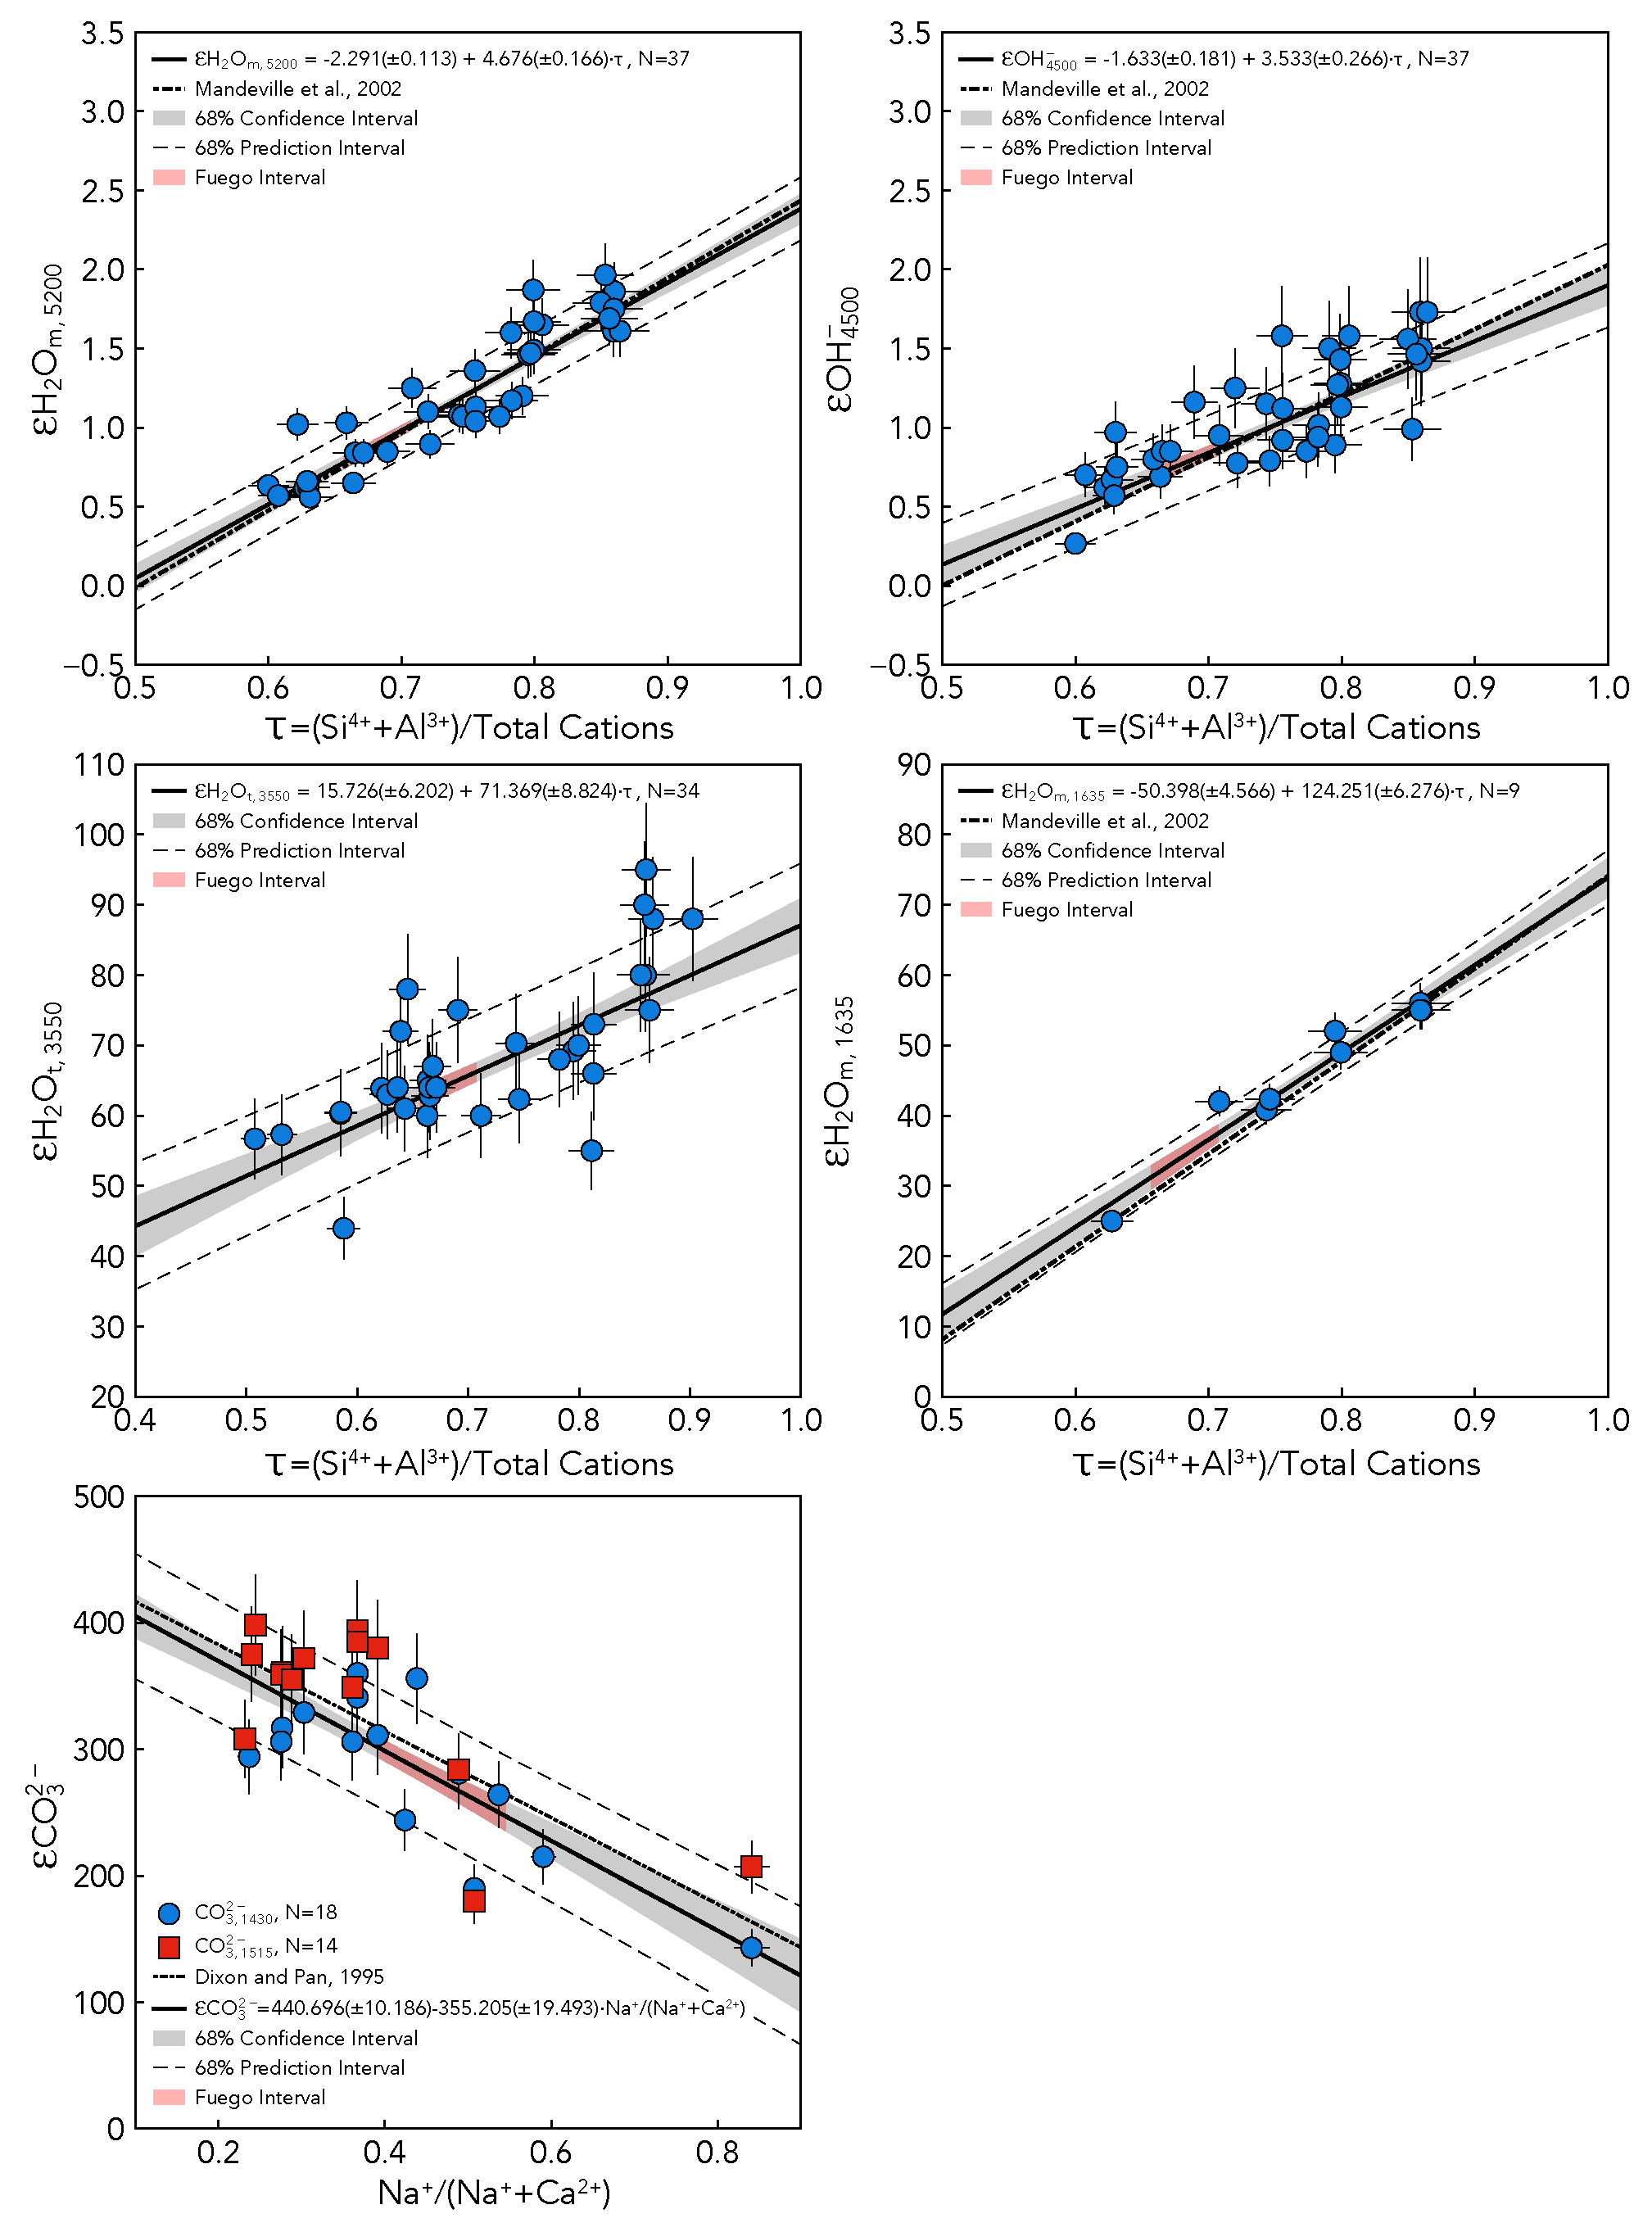
\includegraphics[width=1.0\textwidth]{AllEpsilonRegress}
\caption[Epsilon Regressions]{Epsilon regressions}
\label{figure:EpsilonRegressions}
\end{figure}

%  CALCULATING THICKNESS FROM REFLECTANCE FTIR
\subsection{Calculating Thickness from Reflectance FTIR Spectra}
We develop an automated implementation for calculating thicknesses from reflectance spectra by the interference fringe method. Wavelengths of interference fringes are proportional to the thickness and refractive index of the sample for thin silica films~\cite{Nishikidaetal1996, Tamicetal2001, WysoczanskiandTani2006, Sunetal2007}.~\citeA{Nishikidaetal1996} show the relationship applicable to glasses and olivine: 
\begin{equation}
l = \frac{m}{2n (v_1 - v_2)}
\end{equation}
where $l$ is the thickness of area analyzed, $m$ is the number of fringes in the wavenumber range, $n$ is the refractive index of the material, and $v_1$ and $v_2$ are the highest and lowest wavenumbers in the interval. Interference fringes are produced by the interactions between reflected light and reflections internal to the sample, with fringe wavelengths inversely proportional to thickness. 

Signal-to-noise ratios associated with interference fringes can be low. Reflectance spectra are preprocessed with median filtering to remove potential single spike noise and successively processed with Savitzky-Golay filtering, fitting low-degree polynomials to data with linear least squares~\cite{SavitzkyandGolay1964}. Local extrema associated with each interference fringe wave are located by identifying regions of greatest absorbance change. Maxima are surrounded by points that are lower in absorbance and minima are surrounded by points that are greater in absorbance. Local extrema identification by differentiation can fail with noisier spectra. Thicknesses are calculated from the wavenumber differences between each sequential grouping of local maxima or minima within the inputted wavenumber range. 

Mean thicknesses and standard deviations from local maxima and minima are determined and compared against those from digital micrometer to assess the uncertainty associated with this method. Two to eight interference fringes in the wavenumber range of 1700 to 2850 cm$^{-1}$ for Volcán de Fuego olivines. A refractive index of 1.709 was determined with the average Fo$_{72}$ composition for spots adjacent to melt inclusions with the linear, orientation-dependent parameterization of olivine refractive index from~\citeA{DHZ1992}

Increasing the wavenumber range compared to that of~\citeA{NicholsandWysoczanski2007} increases the number of high-quality interference fringe waves while reproducing digital micrometer measurements. Average thickness uncertainties associated with five measurements is similar to previously reported values at less than 3 \textmu m~\cite{Allisonetal2019, NicholsandWysoczanski2007, vonAulocketal2014}. Thickness by the reflectance fringe method was uniformly greater than that by the digital micrometer, likely suggesting that the olivine refractive index calculated from~\citeA{DHZ1992} is too low. Uncertainties in the refractive index may exist, given the lack of parameterization of composition dependence and the lack of recent analyses.
\textbf{Add stuff on Fuego wafers as proof of concept.}

%  CALCULATING DENSITY
\subsection{Calculating Density}
Melt density is a function of glass composition, and is calculated from the gram formula weight and partial molar volumes (at ambient temperature and pressure of the analytical conditions) from~\citeA{LesherandSpera2015}. The large molar volume of H$_{2}$O significantly impacts density and requires the implementation of an iterative solver. Density is initially assumed to have no contribution from H$_{2}$O but is iteratively update with the calculated amount of H$_{2}$O$_{\mathrm{t, 3550}}$ or H$_{2}$O$_{\mathrm{m, 1635}}$ + OH$^{-}_{4500}$ if the sample is saturated. The \textepsilon${\mathrm{H_2O_{t, 3550}}}$ is analyzed to determine saturation, returning an error message when raw absorbance is \textgreater 2. The H$_{2}$O$_{\mathrm{m}, 1635}$ and OH$^{-}_{4500}$ peaks are used as total H$_{2}$O in determining density when saturated. The density calculation is repeated to ensure stability and converges within 10 iterations. 

%  ALS METHOD
\subsection{Asymmetric Least Squares for H$_{2}$O$_{\mathrm{m}, 5200}$, OH$^{-}_{4500}$, and ${\mathrm{H_2O_{t, 3550}}}$ Peak Heights}

The ${\mathrm{H_2O_{t, 3550}}}$, H$_{2}$O$_{\mathrm{m}, 5200}$, and OH$^{-}_{4500}$ baselines are fit with the asymmetric least squares (ALS) method, iteratively solving for an interpolated fitting which balances smoothness and asymmetry~\cite{Eilers2004, Leeetal2017, Pengetal2010}. \textbf{Look up ALS a bit more, define more properly}. Data are preprocessed by first applying a median filter to remove single spike noise. Three repeat baselines, varying the regions of interest surrounding each peak, are fit with ALS to assess uncertainty within peak height and subtracted from each peak. The three baseline-subtracted peaks are kriged to reduce noise and to obtain maximum peak height. \textbf{Look up kriging a bit more, define more properly}. The mean peak absorbance and standard deviation in absorbance are determined from the repeat baseline-subtracted peaks. ${\mathrm{H_2O_{t, 3550}}}$ saturation prompts the return of an error message and suggestion of use of the H$_{2}$O$_{\mathrm{m}, 5200}$ and OH$^{-}_{4500}$ peaks for determining ${\mathrm{H_2O_{t}}}$

%  MARKOV-CHAIN MONTE CARLO
\subsection{Markov Chain Monte Carlo Algorithm for H$_{2}$O$_{\mathrm{m}, 1635}$ and  CO$_{3}^{2-}$ Doublet}

The net equation describing the absorbance spectrum of a glass or melt inclusion, with \textupsilon$^-$ defined as the wavenumber range from 2400 to 1275 cm$^{-1}$, is thus expressed in the following form:
\begin{eqnarray*}
\hat{A} & = & x_0 \overline{B} + x_1 \overline{B}_{PC1} + x_2 \overline{B}_{PC2} + x_3 \overline{B}_{PC3} + x_4 \overline{B}_{PC4} \\
    && + y_0 \overline{H_2O_{m, 1635}} + y_1 \overline{H_2O_{m, 1635}}_{PC1} + y_2 \overline{H_2O_{m, 1635}}_{PC2} \\
    && + \frac{a_{1515}}{2\sigma_{1515}^2} \cdot e^{-(\upsilon^- - \mu_{1515})^2} + \frac{a_{1430}}{2\sigma_{1430}^2} \cdot e^{-(\upsilon^- - \mu_{1430})^2} +  mv + b 
\end{eqnarray*}
where $x_{0}$, $x_{1}$, $x_{2}$, $x_{3}$, $x_{4}$, $y_{0}$, $y_{1}$, $y_{2}$, $a_{1515}$, $a_{1430}$, $\sigma_{1515}$, $\sigma_{1430}$, $\mu_{1515}$, $\mu_{1430}$, m, and b are the best fit parameters. These fit parameters are first determined by ordinary least squares. The model parameter space of the modeled absorbance of the melt inclusion spectrum is sampled and explored by leveraging a Monte-Carlo Markov Chain algorithm in a Bayesian parametric framework, to account for uncertainty. In this framework of Bayesian inferences, the posterior joint probability distribution of model parameters is quantified as a function of the prior probability of model parameters and a likelihood function. Bayes’ Theorem dictates that the posterior joint probability distribution is updated as more information becomes available, following~\citeA{Cubillosetal2017}: 
\begin{equation}
P(\theta | y, M) \propto P(\theta | M) P(y | \theta, M),
\end{equation}
where $y$ denotes data, $\theta$ is the set of parameters, $P(\theta|y, M)$ is the posterior probability distribution of parameters, $P(\theta|M)$ is the prior probability distribution (not incorporating new information), and $P(y|\theta, M)$ is the likelihood. The prior probability distribution of parameters is defined by the expected range and distributions of these parameters. The likelihood serves as the probability density function of the modeled data given an array of parameters. A Markov-Chain Monte Carlo (MCMC) algorithm was utilized to generate random samples from the parameter space to generate and assess the parameter space, where the random samples generated by the algorithm hold a probability density distribution that is proportional to the posterior probability distribution. The open-source Python package, Multi-Core Markov-Chain Monte Carlo, or MC$^{3}$, integrates these statistical methods~\cite{Cubillosetal2017} and was implemented for this study.

Fixed absorbance spectra provide the information required to generate improved posterior probability distributions of model parameters. Prior probability distributions of the parameters generating the baseline, peaks, and lines require different functions – either uniform or Gaussian – to accurately represent this space. Parameters related to the baselines, H$_{2, m}$O peak, CO$_{3}^{2-}$ doublet peak heights, and linear adjustment are sampled uniformly, given the greater variation within these parameters that is not defined around one value. The exploration space provided these uniformly sampled priors is guided by the initial model generation process. The CO$_{3}^{2-}$ doublet peak locations and standard deviations are defined with a Gaussian prior, given the well-defined nature of these parameters in basaltic melt inclusion absorbance spectra. The initial prior parameters are optimized with the least-squares Trust Region Reflective algorithm, which is suitable for well-constrained, large problems~\cite{Branchetal1999}. 

Random MCMC sampling is performed with the Snooker Updater Differential Evolution Markov Chain method (DEMC), which involves the parallel evolution of multiple chains and computation of appropriate scales and orientations for the jumping distribution~\cite{terBraak2006, terBraakandVrugt2008}. The scale and direction of the proposed jump is computed by the parallel computation of several chains, which allow for the differences between one chain and two additional randomly selected chains to evolve forwards. The chains will converge towards a posterior distribution and will align the evolution along the proper orientation, with good scaling. The Snooker Updater DEMC optimizes acceptance rates and efficiency, allowing for one absorbance spectrum to be run within 15 seconds. 

The Bayesian and MCMC framework underlying this model allows for numerous parameters to be sampled and fit concurrently, while accounting for covariance and quantifying uncertainties. The peak heights and standard deviation of the H$_{2}$O$_{\mathrm{m}, 1635}$ and CO$_{3}^{2-}$ doublet peaks are exported from the algorithm and used to determine volatile concentrations. 

\subsection{Markov Chain Monte Carlo for Calculating Concentration}


The final density obtained following the iteration and appropriate absorption coefficients are applied to the Beer Lambert Law, with the ALS and MC3 determined peak heights, to determine the concentration of total H2O, molecular H2O, and CO2 of each doublet peak. 


The final density, the appropriate absorption coefficient, and the ALS and MC$^3$ determined peak heights of absorbance are applied through the Beer Lambert Law to determine the concentration of H$_{2}$O$_{\mathrm{t}}$, H$_{2}$O$_{\mathrm{m}}$, OH$^{-}$, and CO$_{2}$ of each doublet peak. A standard deviation on each concentration is taken by running a simple Monte Carlo error assessment in which all parameters (except molar mass) are allowed to vary with a normal distribution for 5x10$^{5}$ samples.


%% ------------------------------------------------------------------------ %%
%  ANALYTICAL METHODOLOGY 

\section{Analytical Methodology} % Section - 1.4
%  TRANSMISSION FTIR 
\subsection{Transmission Fourier Transform Infrared Spectroscopy (FTIR)}
Natural glass standards and olivine-hosted melt inclusions (MIs) were analyzed with the Thermo Scientific Nicolet iN10 MX Fourier Transform Infrared (FTIR) Spectrometer at the Lamont-Doherty Earth Observatory. Glass standards and MIs were placed on a CaF$_2$ plate within the sample holder for measurement of IR absorbance during transmission in the detector spectral range of 8000-450 wavenumbers (cm$^{-1}$). The FTIR was purged for twenty minutes to decrease the signal of atmospheric H$_{2}$O and CO$_{2}$. Glasses and MIs were mapped for absorbance to determine potential heterogeneity in volatile concentrations and to determine the boundaries of measurement — particularly for MI to ensure double intersection. Absorbance maps were generated at a point spacing of 10$\times$10 \textmu m, with 16 scans taken at each point at a resolution of 16 cm$^{-1}$. The relatively few scans and low resolution were balanced to yield manageable mapping times of approximately 15 minutes for each MI. Maps guided the selection of optimal regions for volatile analyses. Three repeat measurements were collected for each glass standard or MI, with 256 collection scans at 4 cm$^{-1}$ spectral resolution. Background scans were collected under the same conditions through the CaF$_{2}$ plate. Aperture sizes (30-200 \textmu m for glass standards and 15-50 \textmu m for MIs) were selected to maximize analytical area and to ensure that light propagated solely through the MI without including the host olivine. The Happ-Genzel apodization function within the Thermo-Nicolet OMNIC Picta software was applied to each spectrum to maintain resolution and reduce noise. Three repeat measurements were taken for each MI. Internal standards of submarine arc lava GH88-1-D1010 analyzed by~\citeA{Newmanetal2000} with FTIR and basaltic MIs CN\_C\_OL1’, CN92C\_OL2, and ETF46 analyzed by~\citeA{Barthetal2019} and~\citeA{BarthThesis} with SIMS were measured at the beginning and end of each analytical session as internal check standards. 

%  REFLECTANCE FTIR 
\subsection{Reflectance Fourier Transform Infrared Spectroscopy (FTIR)}
Three repeat thickness measurements of olivine-hosted melt inclusions were acquired using a Mitutoyo 543-783B Digimatic Indicator, as well as with the reflectance method described by~\citeA{NicholsandWysoczanski2007}. Two reflectance spectra were taken adjacent to olivine-hosted melt inclusions with 256 collection scans at 4 cm$^{-1}$ spectral resolution, with aperture sizes of 50$\times$50 \textmu m. Background scans were collected under the same conditions on a highly reflective gold plate with a reflectance coefficient of unity~\cite{NicholsandWysoczanski2007}. The basaltic glass refractive index is quantified to be 1.546~\cite{KumagaiandKaneoka2003}. The rhyolitic glass refractive index is not as well quantified, showing additional variability and spanning the range of 1.48\textless $n$\textless 1.51~\cite{Trogeretal1959, Tamicetal2001}. Refractive indices for glasses of variable composition can be calibrated with the digital micrometer~\cite{DuncanandDasgupta2015, Tamicetal2001}. The olivine mean refractive index, averaged across the three crystallographic axes, is described by forsterite content with linear relationships described in~\citeA{DHZ1992}. 

%  EPMA
\subsection{Electron Probe Microanalyzer (EPMA)}
Major and trace elements in glass and olivine were analyzed by wavelength dispersive X-ray spectroscopy with the Cameca SXFive-TACTIS electron microprobe (EPMA) at the American Museum of Natural History. Calibration was completed with natural and synthetic mineral and oxide standards. Glasses were measured with an accelerating voltage of 15 keV, variable working current of 4 nA, 10 nA, and 40 nA, and spot size of 10 \textmu m. Duplicate MI analyses were collected proximal to the center of the inclusion. Na was measured with a working current of 4 nA with 2 s counting on peak and 20 s on background to minimize Na loss. Other major and trace elements were measured with a working current of 10 nA with 30 s counting on peak and 15 s on background. Fe was analyzed with 20 s counting on peak and 15 s on background. Volatiles S and Cl were measured with an increased working current of 40 nA. Olivines were measured with an accelerating voltage of 15 keV, variable working current of 10 nA and 300 nA, and spot size of 1 \textmu m. Duplicate olivine-host analyses were collected approximately 15 \textmu m from the MI. Mg, Si, and Fe were analyzed with a working current of 10 nA, and all remaining minor and trace elements were analyzed with a working current of 300 nA. \textbf{I can't figure out all the counting times from the files, need a bit of help with this for appendix}. Replicate analyses of the check standard MR:ND-70-01 and secondary standards San Carlos Olivine and VG-2 were performed every 10 analyses. Column conditions and additional assessments of Instrumental drift, precision, and accuracy from analysis of standard analyses are provided in~\ref{supplement:a}. 

%Relative proportions of oxidized and reduced S impacts the S valence state and bond energies, which in turn shifts the wavelength of SK\textalpha-radiation~\cite{CarrollandRutherford1988, WallaceandCarmichael1994}. The S peak position was initially calibrated at the peak position for S$^{6+}$, at 61435 sin\straighttheta, using a standard BaSO$_{4}$. The other endmember position for S$^{2-}$ was calibrated with two basaltic check standards, VG-2 and MR-ND-70-01, at 61470 sin\straighttheta \ (Supplement~\ref{supplement:a}). Several wavescans of Fuego melt inclusions were taken to assess the oxidation state and to determine the appropriate peak position on which to measure S. The Fuego melt inclusion wavescans had near-identical peak locations at 61370 sin\straighttheta{}, indicating that the S peak had shifted towards BaSO$_{4}$ (Supplement~\ref{supplement:a}). The peak position was set at 61370 sin\straighttheta{} to measure all melt inclusions. 


%% ------------------------------------------------------------------------ %%
%  VALIDATION
\section{Validation}

%% ------------------------------------------------------------------------ %%






%% ------------------------------------------------------------------------ %%
%  APPLICATION
\section{Application}

%  PYBASELINES PACKAGE
\subsection{PyBaselines Package and Structure}
PyBaselines can be locally installed with Python versions $\ge$ 3.6 using the command line: 
\begin{lstlisting}[language=Python]
pip install PyBaselines 
\end{lstlisting}
and installed with Google Colab and Binder, two cloud-based Python development environments, where installation occurs within a code cell: 
\begin{lstlisting}[language=Python]
!pip install PyBaselines 
\end{lstlisting}
The PyBaselines package must then be loaded and initialized with: 
\begin{lstlisting}[language=Python]
import PyBaselines as bl
\end{lstlisting}
Functions from PyBaselines are then called with the abbreviated package name, followed by a dot, followed by the function name. The function loading all spectrum files is called as follows: 
\begin{lstlisting}[language=Python]
bl.Load_SampleCSV(args)
\end{lstlisting}
and the function processing each spectrum file is called as follows: 
\begin{lstlisting}[language=Python]
bl.Run_All_Spectra(args)
\end{lstlisting}

\subsection{Volcán de Fuego Melt Inclusions}

%% ------------------------------------------------------------------------ %%





%% ------------------------------------------------------------------------ %%
%  APPENDIX

\appendix
\section{Supplement: EPMA Analytical Conditions, Precision, and Accuracy}

\label{supplement:a}
Analytical precision is quantified as the relative standard deviation (standard deviation of repeat analysis / mean composition of standard during session) of repeated analyses of a secondary standard during an analytical session. Analytical accuracy is quantified as the mean composition of the secondary standard during an analytical session divided by the laboratory value for the standard. Specific acquisition parameters and assessments of analytical precision and accuracy are presented in the following tables. 

\begin{table}[!htbp]
\caption[EPMA analytical conditions, precision, and accuracy]{Assessment of EPMA analytical conditions, precision, and accuracy for analyzed phases including glass and olivine}
\label{table:EPMAConditions}

\begin{subtable}[h]{1\textwidth}
\centering
\textbf{Glass} \\ 
\vspace{5pt}
\begin{adjustbox}{width=1\textwidth, center=1\textwidth}
\begin{tabular}{c c c c c c c c}
\hline 
\multirow{3}{*}{Element} & \multirow{3}{*}{Spectrometer} & \multirow{3}{*}{Crystal} & \multirow{3}{*}{Peak Location} & \multirow{3}{2cm}{\centering Counting Time (s)}  & \multirow{3}{2cm}{\centering Calibration Material} & \multirow{3}{*}{Precision (\%)} & \multirow{3}{*}{Accuracy (\%)}\\ 
\\ 
\\
\hline
Na & Sp1 & LTAP & 46415 & 10 & Jadeite & 2.7 &  \\
Si & Sp4 & TAP & 27741 & 10 & Diopside & 0.5 &  \\
K & Sp2 & PET & 42761 & 10 & KSpK & 13.1 &  \\
Ca & Sp2 & PET & 38389 & 20 & Diopside & 0.9 &  \\
Ti & Sp2 & PET & 31416 & 40 & Rutile & 2.1 &  \\
Mg & Sp4 & TAP & 38515 & 20 & Olivine & 1.5 &  \\
Al & Sp1 & LTAP & 32473 & 30 & Corundum & 0.6 &  \\
P & Sp1 & LTAP & 23949 & 30 & Apatite & 20.0 &  \\
Fe & Sp5 & LIF & 48084 & 60 & Fayalite & 0.6 &  \\
Mn & Sp3 & LLIF & 52199 & 40 & MnMnSp & 6.9 &  \\
Cr & Sp3 & LLIF & 56860 & 20 & CrCrSp3 & 94 &  \\
\hline 
\end{tabular}
\end{adjustbox}
\vspace{3pt}
\end{subtable}

\begin{subtable}[h]{1\textwidth}
\centering
\textbf{Olivine} \\ 
\vspace{5pt}
\begin{adjustbox}{width=1\textwidth, center=1\textwidth}
\begin{tabular}{c c c c c c c c}
\hline 
\multirow{3}{*}{Element} & \multirow{3}{*}{Spectrometer} & \multirow{3}{*}{Crystal} & \multirow{3}{*}{Peak Location} & \multirow{3}{2cm}{\centering Counting Time (s)}  & \multirow{3}{2cm}{\centering Calibration Material} & \multirow{3}{*}{Precision (\%)} & \multirow{3}{*}{Accuracy (\%)}\\ 
\\ 
\\
\hline
C1 &  &  &  &  &  & & \\
Si & Sp4 & TAP & 27741 & 10 & Diopside & 0.4&  \\
Fe & Sp3 & LLIF & 48084 & 10 & Fayalite & 1.0 &  \\
Mg & Sp1 & LTAP & 38530 & 10 & Olivine & 0.2 &  \\
C2 &  &  &  &  &  & & \\
Ca & Sp2 & PET & 38389 & 60 & Diopside & 4.4 &  \\
Ti & Sp2 & PET & 31416 & 90 & Rutile & 36.5 &  \\
Cr & Sp5 & LIF & 56866 & 60 & CrCrSp3 & 10.6 &  \\
Mn & Sp5 & LIF & 52205 & 90 & MnMnSp3 & 3.1 &  \\
Ni & Sp3 & LLIF & 41167 & 150 & NiONiSp3 & 0.4 &  \\
Al & Sp1 & LTAP & 32473 & 150 & Corundum & 4.2 &  \\
P & Sp4 & TAP & 23958 & 150 & Apatite & 148 &  \\
\hline 
\end{tabular}
\end{adjustbox}
\vspace{3pt}
\end{subtable}

\end{table}
%% ------------------------------------------------------------------------ %%




%% ------------------------------------------------------------------------ %%
% ACKNOWLEDGMENTS. The acknowledgments must list: A statement that indicates to the reader where the data supporting the conclusions can be obtained (for example, in the references, tables, supporting information, and other databases). All funding sources related to this work from all authors. Any real or perceived financial conflicts of interests for any author. Other affiliations for any author that may be perceived as having a conflict of interest with respect to the results of this paper. It is also the appropriate place to thank colleagues and other contributors. AGU does not normally allow dedications.

\acknowledgments
Enter acknowledgments, including your data availability statement, here.


%% ------------------------------------------------------------------------ %%
%  References and Citations

\bibliography{references}

%% ------------------------------------------------------------------------ %%

\end{document}